\section{Métodos Propuestos}

\subsection{Fast DPP}

El primer algoritmo de esta sección, que denominaremos \textit{Fast DPP}, es la primera modificación al propuesto en \cite{https://doi.org/10.48550/arxiv.1804.02772} y descrito en el capítulo anterior. Este, sienta las bases de los algoritmos propuestos más adelante y busca realizar el entrenamiento de la red neuronal sin la necesidad de mirar todos los datos en cada época, pero intentando siempre maximizar la diversidad de los \textit{batches} sampleados mediante un DPP.

\begin{figure}[ht]
    \centering
    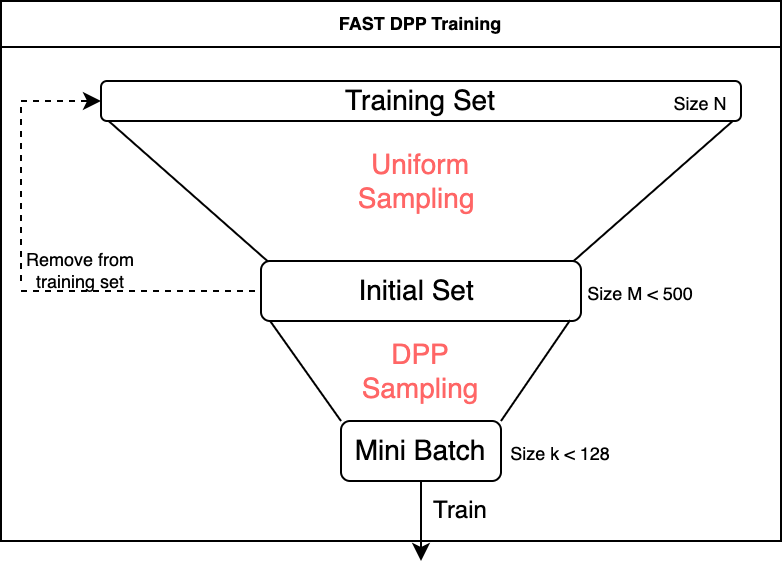
\includegraphics[width=9cm]{img/tesis/fast_dpp_diagram.png}
    \caption{Fast DPP: El diagrama muestra el proceso de extracción de un \textit{Mini Batch} desde el conjunto de entrenamiento y su posterior muestreo con DPP.}
    \label{fig:fast_dpp}
\end{figure}

Como lo muestra la Figura (\ref{fig:fast_dpp}), en cada iteración de una época, se extrae de manera uniforme, un conjunto inicial de cardinalidad $M < 500$ del cual se samplea posteriormente el \textit{mini-batch} de tamaño $k < 128$ haciendo uso del DPP, lo elementos no utilizados se eliminan del conjunto de entrenamiento. La razón por la cual se realiza esta primera selección, es la de reducir el coste de sampling de un DPP y según el parámetro $M$, controlar la cantidad de iteraciones que el algoritmo realiza en la época (a mayor $M$ menos iteraciones por época pero menor será la cantidad de ejemplos visitados y mayor será el tiempo de sampling del DPP).   

\vspace{0.2cm}

Notar que si bien podrían eliminarse del conjunto de entrenamiento únicamente los ejemplos utilizados en el \textit{mini-batch} (y no $M$ completamente), nuestro objetivo es el de acelerar el entrenamiento de la red mediante la omisión de ejemplos ``redundantes'' según el DPP, vale decir, asumir que el \textit{mini-batch} ``resume'' la información contenida en el conjunto $M$.

\begin{algorithm}
\caption{Fast DPP Training por época} \label{alg:alg4}
\begin{algorithmic}
\Require Conjunto de entrenamiento $\{ (x_i,y_i) \}_{i=1}^N$, $M$ tamaño del primer sampling y $k$ tamaño del mini-batch, $k < M$.  

\State $Z \gets \{x_i\}_{i=1}^N$
\While{$|Z| > 0$}

\If{$|Z| > M$}

\State $D \gets$ Sampling uniforme de $Z$, $|D| = M$
\State $B \gets$ Sampling de un DPP de $D$, $|B| = k$ 

\Else

\State $D \gets Z$
\State $B \gets$ Sampling de un DPP de $D$, $|B| = \min(k, |D|)$ 

\EndIf

\State Entrenar la red con el mini-batch $B$

\State $Z \gets Z - D$

\EndWhile   
\end{algorithmic}
\end{algorithm}

Es directo ver que el Algoritmo \ref{alg:alg4} siempre termina pues $D \neq \emptyset$ y la actualización $Z \gets Z - D$ reduce el tamaño de $Z$ hasta que el conjunto es eventualmente vacío. La cantidad de iteraciones por época está dado por $\lfloor N / M \rfloor$ si $M$ es divisor de $N$ y $\lfloor N / M \rfloor + 1$ si no lo es, por lo que comparado a un algoritmo clásico de descenso de gradiente estocástico que realiza $\lfloor N / k \rfloor$ iteraciones o bien $\lfloor N / k \rfloor + 1$, \textit{Fast DPP} realiza aproximadamente $\lfloor M / k \rfloor$ veces menos iteraciones.


\subsection{Mixed DPP}\label{section:mixed_dpp}

La estrategia mencionada anteriormente puede ser de gran utilidad para el entrenamiento de una red neuronal cuyo costo por iteración es elevado. Lamentablemente, el rendimiento de la red \textit{Fast DPP} a lo largo de las épocas no mejora tanto como lo haría un algoritmo que pasa por todos los datos.

\vspace{0.2cm}

Con el objetivo de acelerar el entrenamiento y no sacrificar desempeño, es posible realizar un esquema mixto de entrenamiento que denominamos \textit{Mixed DPP}. Este esquema consta de estrategias de sampleo condicionadas a la época en que se encuentre el entrenamiento, vale decir, es posible utilizar una estrategia \textit{Fast DPP} en las primeras épocas (``inicialización'') del entrenamiento y terminar con un algoritmo de SGD estándar que visite todos los datos o viceversa (\textit{Reversed Mixed DPP}). 

\begin{algorithm}[ht]
\caption{Mixed DPP Training}\label{alg:alg5}
\begin{algorithmic}
\Require Conjunto de entrenamiento $\{(x_i,y_i) \}_{i=1}^N$, $M$ tamaño del primer sampling y $k$ tamaño del mini-batch, $k < M$, $l$ cantidad de épocas de entrenamiento y $l_m$ época de cambio de estrategia , $l_m < l$. 
\For{$e$ in $\{ 1 , \dots l \}$}
\If{$e < l_m$}
\State Entrenar la red con $\text{ALG}_4(\{(x_i,y_i)\}_{i=1}^N , M, k)$
\Else
\State Entrenar la red con $\text{SGD}(\{(x_i,y_i) \}_{i=1}^N,k)$
\EndIf
\EndFor
\end{algorithmic}
\end{algorithm}

\begin{algorithm}[ht]
\caption{Reversed Mixed DPP Training}\label{alg:alg6}
\begin{algorithmic}
\Require Conjunto de entrenamiento $\{(x_i,y_i) \}_{i=1}^N$, $M$ tamaño del primer sampling y $k$ tamaño del mini-batch, $k < M$, $l$ cantidad de épocas de entrenamiento y $l_m$ época de cambio de estrategia , $l_m < l$. 
\For{$e$ in $\{ 1 , \dots l \}$}
\If{$e > l_m$}
\State Entrenar la red con $\text{ALG}_4(\{(x_i,y_i)\}_{i=1}^N , M, k)$
\Else
\State Entrenar la red con $\text{SGD}(\{(x_i,y_i) \}_{i=1}^N,k)$
\EndIf
\EndFor
\end{algorithmic}
\end{algorithm}

\vspace{0.2cm}

La idea de \textit{Mixed DPP} es que permite ``mapear'' de manera acelerada las regiones de decisión del problema de clasificación en las primeras épocas y terminar el entrenamiento realizando ligeros ``ajustes'' utilizando un SGD clásico. Se añade además \textit{Reversed Mixed DPP}, que es la idea contraria a \textit{Mixed DPP} pues es en las últimas épocas de entrenamiento (cuando la función de \textit{loss} ya no varía mucho), en la que se aplica \textit{Fast DPP} con la intención de superar el \textit{plateau} al cambiar la distribución de los \textit{batches}. 

%con la idea de que en las últimas épocas de entrenamiento, cuando la función de \textit{loss} ya no varía, el método pueda superar el \textit{plateau}.

\vspace{0.2cm}

Ambas estrategias Algoritmo \ref{alg:alg5} y Algoritmo \ref{alg:alg6} son más rápidas que entrenar con un algoritmo $SGD$ clásico pues optimizan el tiempo de entrenamiento en las épocas con \textit{Fast DPP}. 

\subsection{DPP NET}

Este modelo propuesto intenta solucionar el problema de la definición de la métrica de similitud necesaria para samplear un DPP mientras se entrena en simultaneo la red que se encarga del problema de clasificación. 

\begin{figure}[ht]
    \centering
    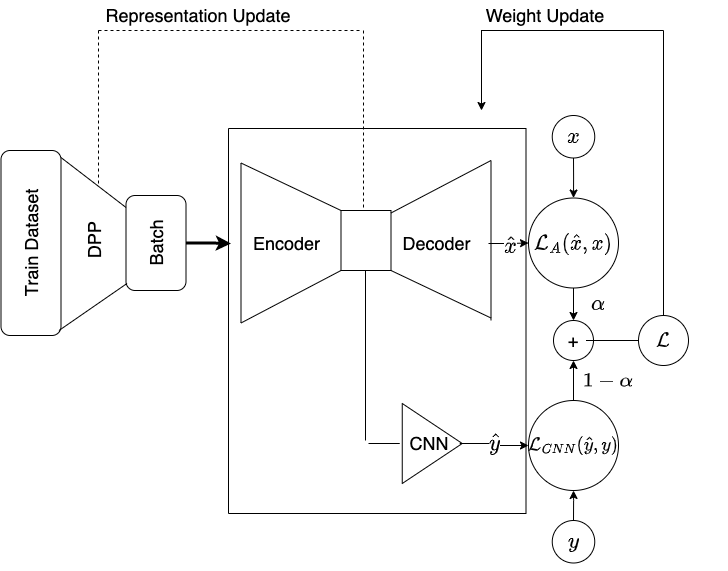
\includegraphics[width=10cm]{img/tesis/dpp_net.png}
    \caption{DPP NET: El diagrama muestra una arquitectura que incluye el muestreo mediante un DPP, el \textit{Autoencoder} encargado de obtener la representación de baja dimensionalidad de los datos y la subred encargada de la predicción de la etiqueta del problema de clasificación.}
    \label{fig:dpp_net}
\end{figure}

\vspace{0.2cm}

La red se compone principalmente de un \textit{Autoencoder} y una \textit{fully connected} (FC) o una red convolucional (CNN). La sección del \textit{Encoder} junto a la FC (o CNN), se encargan de realizar la predicción de la etiqueta del problema de clasificación. Por otro lado, el \textit{Autoencoder} en simultaneo, estima una representación de menor dimensionalidad del \textit{input} que servirá para los futuros muestreos del DPP con el uso de una distancia euclidiana. Para entrenar la red, se utiliza la siguiente función de \textit{loss}

\[
\mathcal{L} = \alpha\mathcal{L}_A(\hat{x},x) + (1-\alpha)\mathcal{L}_{CNN}(\hat{y},y) , 
\] es decir, una suma ponderada de las \textit{losses} del \textit{Autoencoder} y de la subred encargada del problema de clasificación como lo muestra el Diagrama \ref{fig:dpp_net}.

\vspace{0.2cm}

La ventaja de este enfoque es que no requiere del entrenamiento previo del \textit{Autoencoder} o del aprendizaje de la métrica con \textit{Oneshot Learning}. Por otro lado, con el parámetro $\alpha$, es posible controlar qué tanto se busca actualizar los pesos de ambas redes por separado y de ser necesario, desconectar una de otra. 

\vspace{0.2cm}

El desafío de este modelo es que el entrenamiento en comparación con un \textit{baseline} de arquitectura equivalente pero que no entrene un \textit{Autoencoder}, es el tiempo por iteración necesario para su ajuste. Por tanto, será importante ajustar el valor de $M$ en \textit{Fast DPP} con tal de no perder en rendimiento ni en tiempo de entrenamiento. 

\begin{algorithm}
\caption{DPP NET por época}\label{alg:alg7}
\begin{algorithmic}
\Require Conjunto de entrenamiento $\{(x_i,y_i) \}_{i=1}^N$, $M$ tamaño del primer sampling y $k$ tamaño del mini-batch, $k < M$, $\alpha \in [0,1]$ 

\State $Z \gets \{x_i\}_{i=1}^N$
\While{$|Z| > 0$}

\If{$|Z| > M$}

\State $D \gets$ Sampling uniforme de $Z$, $|D| = M$
\State $\hat{D} \gets \text{Encoder}(D)$
\State $B \gets$ Sampling de un DPP de $\hat{D}$, $|B| = k$  

\Else

\State $D \gets Z$
\State $\hat{D} \gets \text{Encoder}(D)$
\State $B \gets$ Sampling de un DPP de $\hat{D}$, $|B| = \min(k, |\hat{D}|)$ 

\EndIf

\State Entrenar la red con el mini-batch $B$ y \textit{loss} $\mathcal{L} = \alpha\mathcal{L}_A(\hat{x},x) + (1-\alpha)\mathcal{L}_{FC}(\hat{y},y) $ 

\State $Z \gets Z - D$

\EndWhile  
\end{algorithmic}
\end{algorithm}

\section{Definición de Métricas}


\subsection{Kernel RBF}

Recordemos que para samplear de un DPP es necesario un kernel $K$ (o un L-ensamblaje) que cumpla con ser semidefinido positivo y de valores propios acotados por 1. Por otro lado, si se asume que todos los elementos de un conjunto son equiprobables de samplear, la diagonal del kernel debe tener valores iguales, es decir $K_{i,i} = c > 0 , \forall i$.

\vspace{0.2cm}

Con lo anterior, un kernel que cumple con tales características es el kernel RBF (Radial Basis Function) \cite{article2} definido como 
\[
K(x_i, x_j) = \exp \left ( - \frac{d(x_i,x_j)^2}{2l^2}\right ) , 
\]
donde $d(\cdot,\cdot)$ es alguna métrica de distancia y $l>0$ el \textit{length scale}. Notar que $d(x_i, x_i) = 0 \Rightarrow K(x_i,x_i) = 1$ y si $d(x_i , x_j) \rightarrow \infty \Rightarrow K(x_i,x_j) \rightarrow 0$ lo que hace sentido pensando en que en los procesos repulsivos $\mathcal{P}$ samplean con mayor probabilidad elementos alejados unos de otros ya que 
\[
\mathcal{P}(i,j \in Y) = \mathcal{P}(i \in Y)\mathcal{P}(j \in Y) - K_{ij}^2 .
\]

\subsection{Minkowski de orden $p$}\label{section:minkowski}

La principal dificultad de trabajar con un proceso repulsivo como un DPP es definir correctamente la métrica de similitud (o distancia) $d(\cdot,\cdot)$. Esto pues, dependiendo del tipo de dato ya sean imágenes, series de tiempo, textos, entre otros, la métrica más adecuada puede variar entre los problemas. 

\vspace{0.2cm}

Para abordar el problema, se puede suponer que el tipo de dato es un vector $x \in \mathbb{R}^d$ donde generalmente $d \in \mathbb{N}$ es grande ($d\geq9$). Es posible utilizar $d(x,y) = ||x-y||_2$ la distancia euclidiana como medida de similaridad pero no es tan efectiva en altas dimensiones como lo muestra \cite{https://doi.org/10.1002/sam.11161} por lo que se propone alternativamente utilizar la generalización
\[
d_p(x,y) = ||x-y||_p = \left (\sum_{i=1}^d |x_i-y_i|^p\right)^{1/p}, 
\]
llamada distancia de \textit{Minkowski} de orden $p$. Si $p=2$ se obtiene la distancia euclidiana, si $p=1$ se obtiene la distancia de \textit{Manhattan} y si $p<1$ se obtiene la ``distancia'' fraccional que si bien no cumple exactamente la desigualdad triangular, son menos propensas a sufrir el efecto de ``concentración'' que tiene la distancia euclidiana en altas dimensiones y por tanto son útiles para este tipo de problemas \cite{10.1007/3-540-44503-X_27}. 


\begin{figure}[ht]
    \centering
    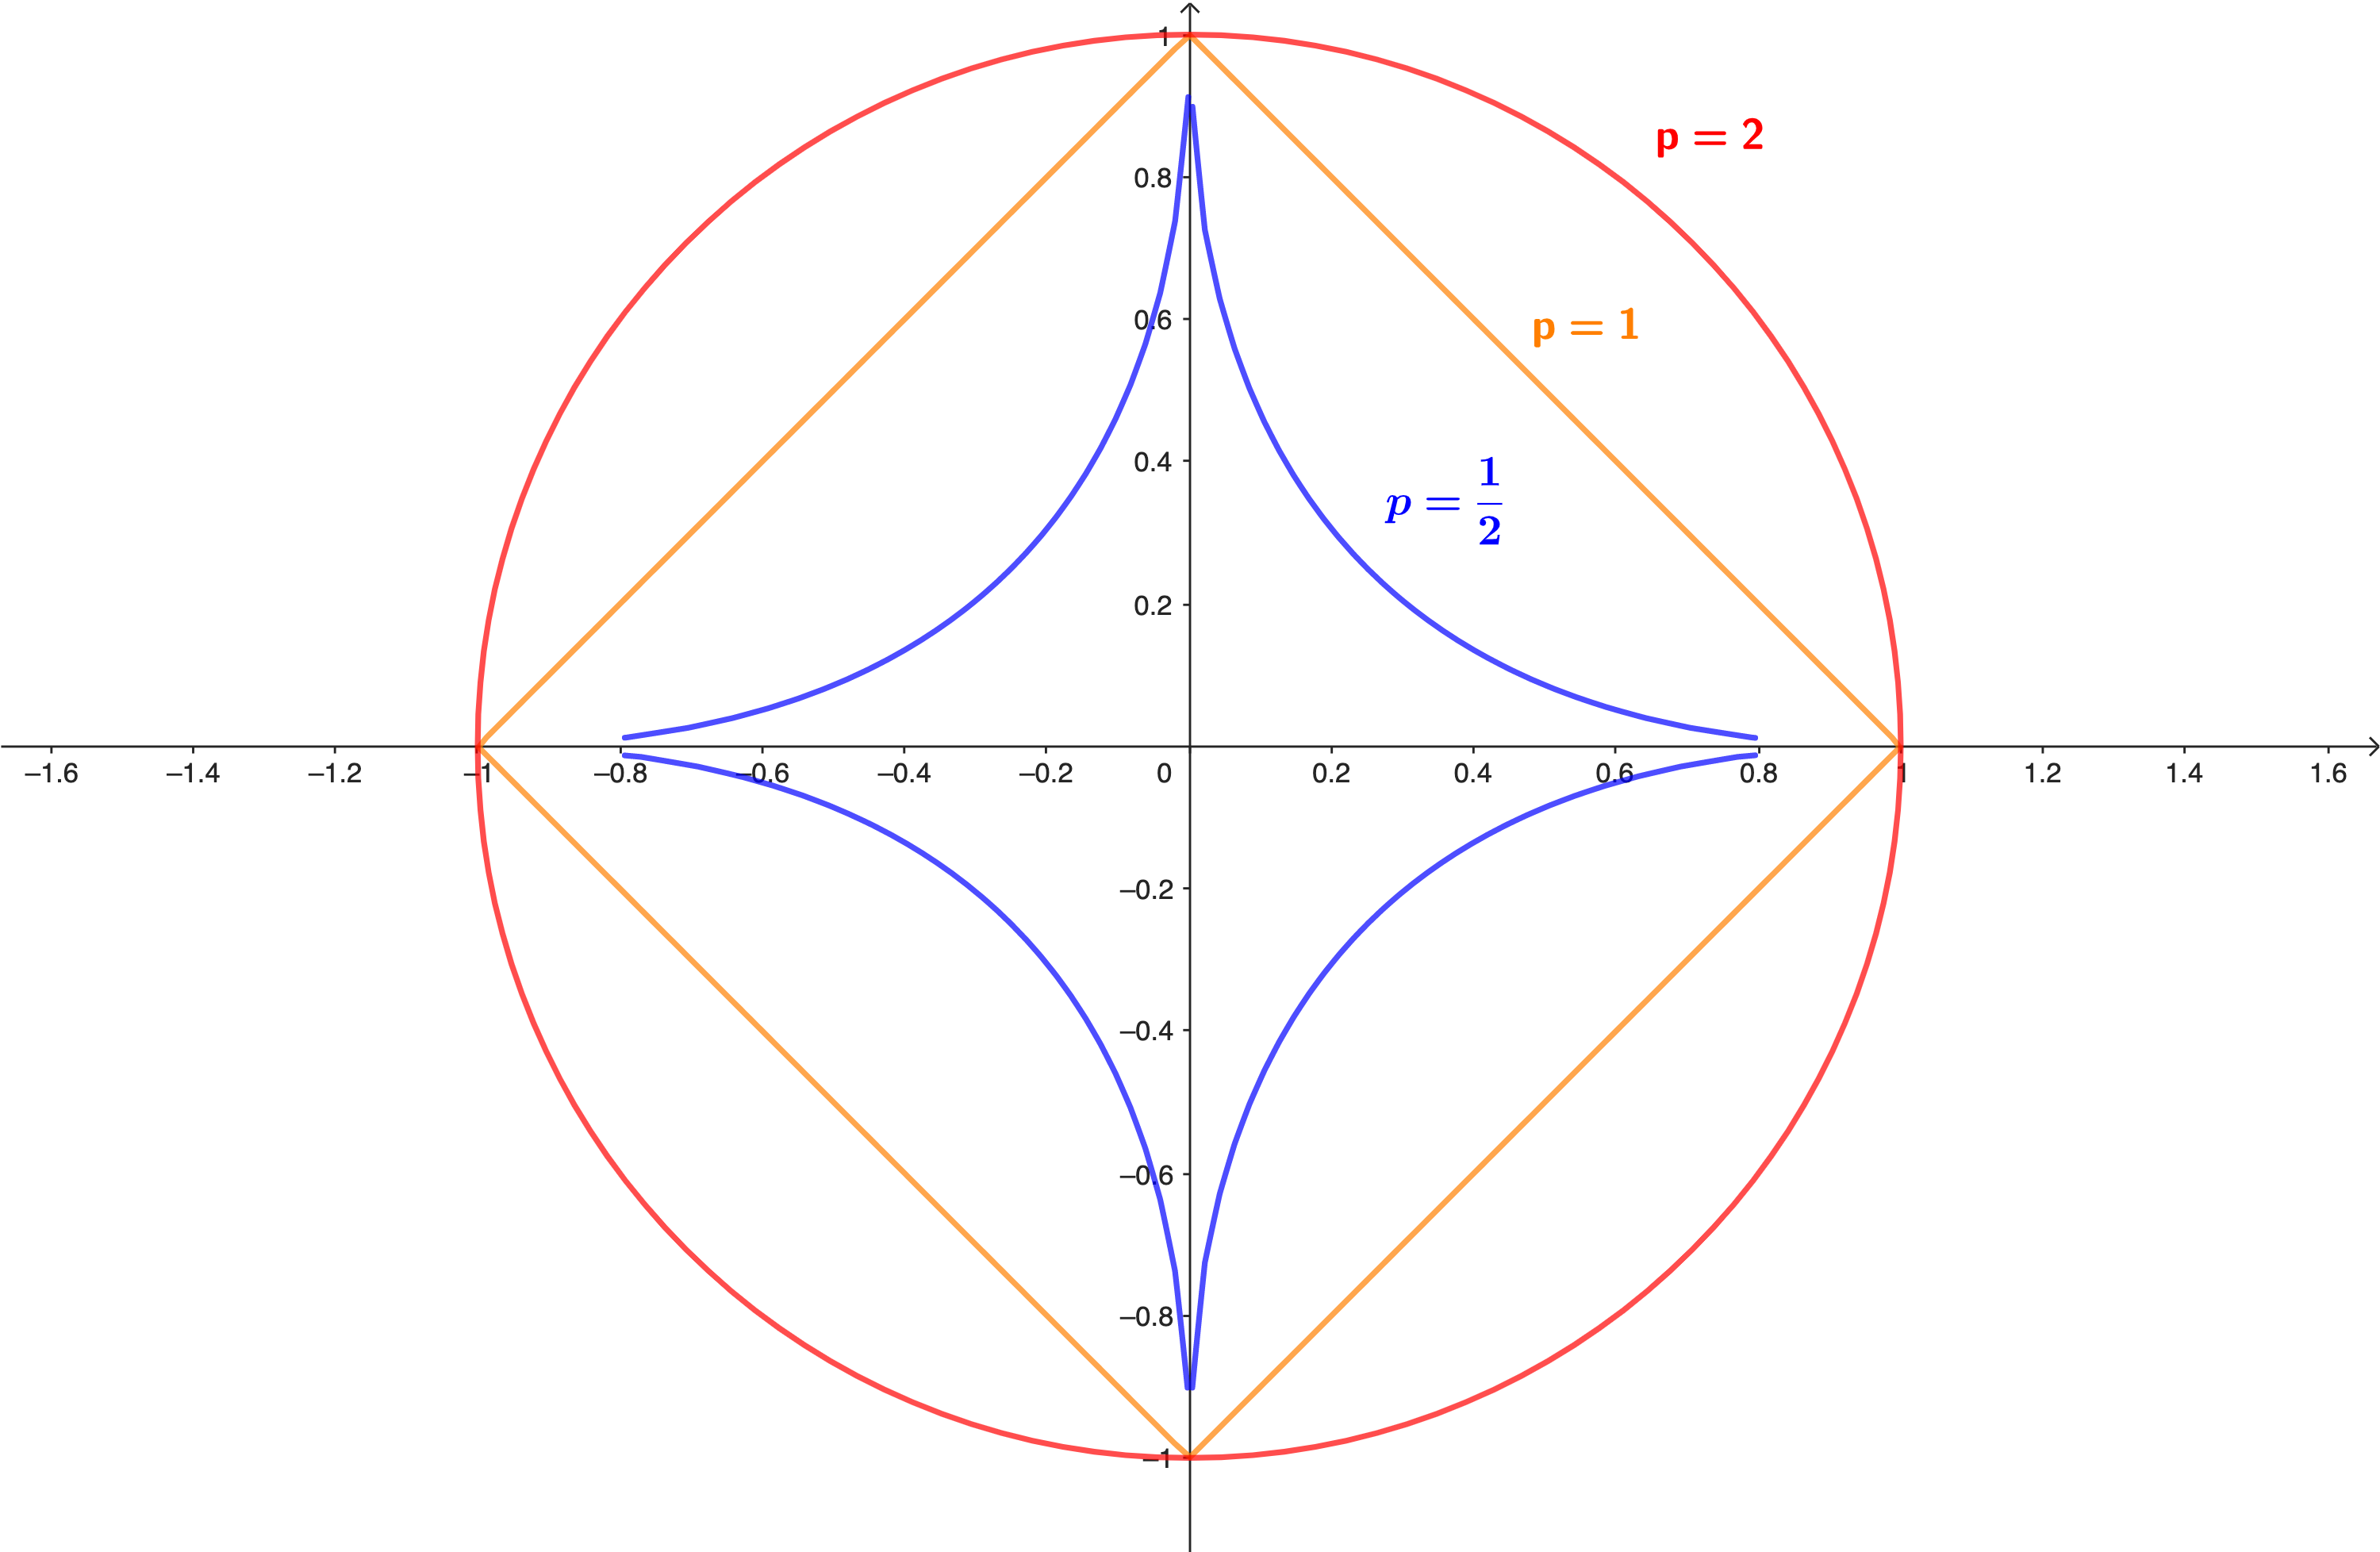
\includegraphics[width=9cm]{img/tesis/bola_unitaria.png}
    \caption{Bola Unitaria para distintos valores de $p$.}
    \label{fig:2d_unit_balls}
\end{figure}

\subsection{Distancia Coseno}

Otra métrica relevante a considerar es la ``distancia'' coseno definida como 
\[
d_{\text{cos}}(x,y) = 1 - \text{sim}_{\text{cos}}(x,y) = 1 - \frac{\langle x,y \rangle}{||x||_2||y||_2} , 
\]
notar que si bien no cumple con la desigualdad triangular, esta métrica es de utilidad para diferenciar elementos según su dirección con respecto al origen y no según la magnitud como la distancia euclidiana. Lamentablemente, esta métrica se ve afectada por la maldición de la dimensionalidad aunque en menor magnitud. 


\subsection{Autoencoder: Representación Latente}

La utilización de un \textit{Autoencoder} resulta de gran utilidad para definir una métrica de distancia que no dependa en gran medida del tipo de datos con los que se trabaja. Al obtener la representación de baja dimensionalidad de los datos, la distancia euclidiana o coseno representan de manera fidedigna la similitud de los datos y por tanto pueden ser utilizados por el DPP. De manera formal 

\[
d_{auto} = || \text{encoder}(x) - \text{encoder}(y) ||_2 .
\]

Lamentablemente, es necesario ajustar un \textit{Autoencoder} previo al entrenamiento de la red encargada de resolver el problema de clasificación y esto podría traer aumentos de tiempo importantes a considerar. Las posibles soluciones son la combinación de entrenamientos o el uso de redes pre-entrenadas para este propósito.   

\subsection{Learned Metric: One Shot Learning}

Este tipo de métrica es resultado directo del entrenamiento de una red siamesa descrita en el capítulo 2 y que, al igual que un \textit{Autoencoder}, utiliza una representación latente de los ejemplos para determinar su similitud con una distancia euclidiana. La ventaja de este enfoque es que el \textit{output} de la red es efectivamente una métrica de distancia (\textit{Learned Metric}) y que además requiere de unos pocos ejemplos para ser entrenada. 

\section{Métrica de Desempeño}

El tipo de problema en que nos centraremos corresponden a problemas de clasificación (binarios y multiclase), es decir, donde el \textit{output} $Y$  es una variable cualitativa discreta. Se define el \textit{accuracy} como

\[
\text{accuracy}(y_{pred}, y_{real}) = \frac{TP + TN}{TP + TN + FP + FN} , 
\]
donde TP = Verdaderos positivos, TN = Verdaderos Negativos, FP = Falsos Positivos y FN = Falsos Negativos. Si bien podríamos utilizar esta métrica para medir el desempeño de la red, lo anterior no toma en consideración los ajustes sobre la región de decisión que no cambian la clasificación de los ejemplos pero que si los diferencia con mayor certeza. Dado lo anterior, se decide utilizar directamente la métrica que calcula la función de \textit{loss} en problemas de clasificación 
\[
\mathcal{L} = - \sum_{i=1}^C t_i \log(p_i) , 
\]
donde $C$ es el total de clases, $t_i$ es la etiqueta real del ejemplo y $p_i$ es la probabilidad de pertenecer a la clase $i$ (calculada con una función \textit{sigmoid} en el caso binario y con una función \textit{softmax} en el caso multiclase). Esta métrica permite notar diferencias en el desempeño de una red incluso cuando todos los ejemplos del conjunto son clasificados con las mismas etiquetas que en una iteración anterior. 

\section{Conjuntos de Datos}

Se presenta a continuación los datasets que serán utilizados para los experimentos de la sección posterior.

\subsection{Clasificación Binaria - Baja Dimensionalidad}

El dataset de clasificación binaria \textit{dummy} busca recrear una situación en que los datos de 2 grupos se encuentran en forma de ``clusters'' donde uno de ellos posee considerablemente menos ejemplos.

\begin{figure}[ht]
    \centering
    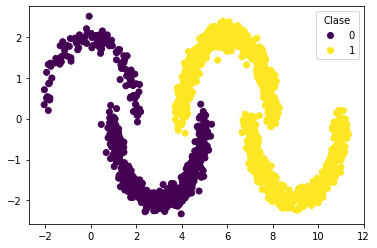
\includegraphics[width=8cm]{img/tesis/binario.png}
    \caption{Dataset de Clasificación Binaria con 4 clusters artificiales y desbalanceados en forma de luna.}
    \label{fig:binaria}
\end{figure}

\begin{table}[ht]
\begin{tabular}{|c|c|c||c|}
\hline
Clase / Cluster & Cluster Superior & Cluster Inferior & Total \\ \hline
Clase 0         & 120 (6.66\%)              & 480 (26.66\%)  & 600 (33.33\%)  \\ \hline
Clase 1         & 600 (33.33\%)             & 600 (33.33\%)  & 1200 (66.66\%)            \\ \hline
\end{tabular}
\caption{Ejemplos por Cluster - Clasificación Binaria. Total = 1800.}
\label{table:binaria}
\end{table}

El objetivo de esta configuración es el de permitir que el DPP samplee con mayor frecuencia los ejemplos del cluster que se encuentra en minoría frente al resto.

\subsection{Clasificación Multiclase - Alta Dimensionalidad}

El dataset de clasificación multiclase \textit{Fashion MNIST} en Figura (\ref{fig:fashion_mnist}) abarca el problema de clasificación multiclase (10 clases) de distintas prendas de ropa. 

\begin{figure}[ht]
    \centering
    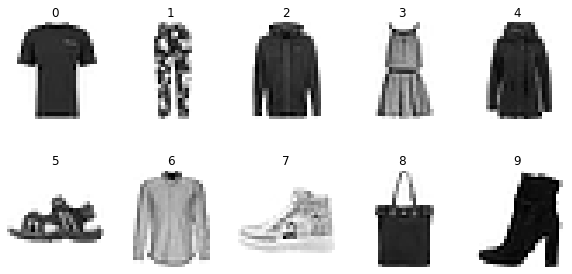
\includegraphics[width=8cm]{img/tesis/fashion_mnist.png}
    \caption{Ejemplos de las 10 clases presentes en el conjunto de datos Fashion-MNIST.}
    \label{fig:fashion_mnist}
\end{figure}

\vspace{0.2cm}

Notar que al igual que en el dataset anterior, dentro de una misma clase es posible encontrar distintos ``clusters'' correspondiente a la misma prenda de ropa pero con diferencias sustanciales (\ref{fig:fashion_mnist_label_3}).

\vspace{0.2CM}

\begin{figure}[ht]
    \centering
    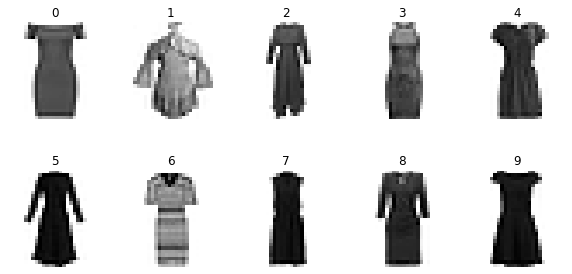
\includegraphics[width=8cm]{img/tesis/fashion_mnist_label_3.png}
    \caption{Ejemplos de la Clase 3 del conjunto de datos Fashion - MNIST.}
    \label{fig:fashion_mnist_label_3}
\end{figure}

Con el fin de agregar complejidad al problema, se utilizará una versión desbalanceada del dataset como la muestra (\ref{table:fashion_mnist}).

\begin{table}[ht]
\begin{tabular}{|c|c|c|c|c|c|c|c|c|c|c|}
\hline
Clase    & 0    & 1    & 2    & 3    & 4    & 5    & 6   & 7   & 8   & 9   \\ \hline
Cantidad & 2500 & 2500 & 2500 & 2500 & 1500 & 1500 & 1500 & 500 & 500 & 500 \\ \hline
(\%) & 15.62 & 15.62 & 15.62 & 15.62 & 9.37 & 9.37 & 9.37 & 3.13 & 3.13 & 3.13 \\ \hline
\end{tabular}
\caption{Conjunto de Entrenamiento - Clasificación Multiclase. Total = 16000.}
\label{table:fashion_mnist}
\end{table}

\section{Experimentos}

\subsection{Sampling de la Clase Minoritaria}\label{experiment:sampling}

El primer experimento consiste en mostrar la implementación del Proceso Puntual Determinantal (DPP) y ejemplificar su acción al momento de samplear sobre conjuntos de datos desbalanceados. Para ello, consideraremos el conjunto de clasificación binaria en 2 dimensiones utilizando la distancia euclidiana junto a un kernel RBF como medida de similitud y se realizarán múltiples sampleos con reposición con el objetivo de comparar la distribución resultante. A continuación, se utilizará el conjunto de clasificación multiclase desbalanceado para mostrar los mismos resultados pero comparando la distancia euclidana con las métricas propuestas anteriormente \textit{Coseno}, \textit{Autoencoder}, \textit{Oneshot}. Se excluye del análisis la distancia \textit{Minkoswki} $p<1$ pero se propone como trabajo a futuro.

\subsection{Fast DPP}\label{experiment:fast_dpp}

En esta sección, se compara el rendimiento de la red implementada \textit{Fast DPP} contra un \textit{baseline} de igual arquitectura pero distinta estrategia de sampleo (SGD) en los conjuntos de datos presentados anteriormente. Las arquitecturas utilizadas son descritas en la siguiente sección, las métricas de distancia se utilizarán según los resultados del experimento anterior. El objetivo del experimento es comparar el \textit{performance} de ambas estrategias tanto numérica como visualmente con el fin de justificar las metodologías propuestas en esta tesis. 

\subsection{Mixed DPP}\label{experiment:mixed_dpp}

El experimento en esta sección es análogo en estructura al realizado en \textit{Fast DPP} pues busca comparar el rendimiento de la red propuesta contra un \textit{baseline} de igual arquitectura pero estrategia de sampleo estándar (SGD) en los datasets presentados. A diferencia del experimento anterior, ahora se entrena por una mayor cantidad de épocas con el fin de determinar si samplear con alguna estrategia distinta en el principio (\textit{Mixed DPP}) o al final (\textit{Reversed Mixed DPP}) resulta en alguna mejora al modelo. 

\vspace{0.2cm} 

\subsection{DPP NET}\label{experiment:dpp_net}

En este último experimento, se busca expandir la metodología descrita en las secciones anteriores mediante el entrenamiento en paralelo del \textit{Autoencoder} necesario para obtener la representación de baja dimensionalidad de los ejemplos del dataset \textit{Fashion MNIST}. Si bien se compara esta nueva red con un \textit{baseline} de arquitectura ``equivalente'', el objetivo es medir el ajuste de la propia red y si es viable para su utilización con un \textit{DPP}. Esto permitiría poder trazar líneas de desarrollo posteriores a esta tesis que serán detalladas en la última sección de conclusiones. La arquitectura a utilizar se describe en la siguiente sección, al igual que los parámetros utilizados. 


\section{Arquitecturas}

Se describen a continuación, el detalle de cada una de las arquitecturas de las redes neuronales utilizadas para los experimentos descritos previamente. 

\subsection{Baseline}

\begin{figure}[ht]
    \centering
    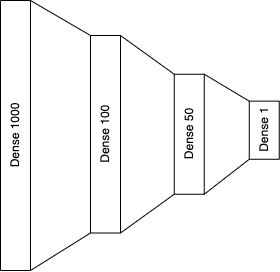
\includegraphics[width=6cm]{img/tesis/baseline_2D.drawio.png}
    \caption{Baseline Clasificación Binaria: Esta arquitectura se utiliza como base para realizar comparaciones de las metodologías propuestas en los problemas de clasificación binaria.}
    \label{fig:baseline_2d}
\end{figure}

\begin{figure}[ht]
    \centering
    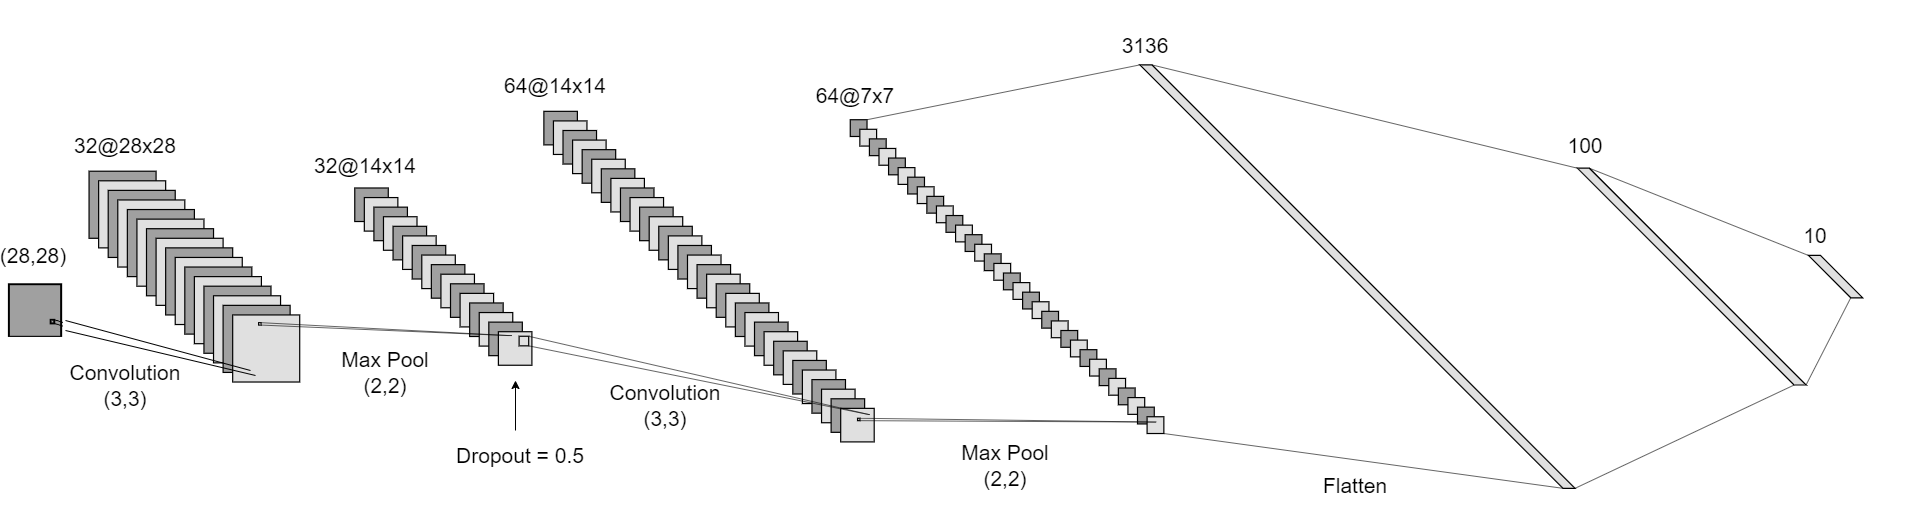
\includegraphics[width=15cm]{img/tesis/conv.drawio.png}
    \caption{Baseline Clasificación Multiclase: Esta arquitectura se utiliza como base para realizar comparaciones de las metodologías propuestas en los problemas de clasificación multiclase.}
    \label{fig:conv}
\end{figure}

Las Figuras \ref{fig:baseline_2d} y \ref{fig:conv} muestran la arquitectura sobre la cual se comparan los métodos propuestos para los problemas de clasificación binaria y multiclase con \textit{Fashion MNIST}. Los parámetros de entrenamiento de ambas se detallan en \ref{table:baseline2d_parameters} y \ref{table:conv_parameters} respectivamente. 

\subsection{Autoencoder}

\begin{figure}[ht]
    \centering
    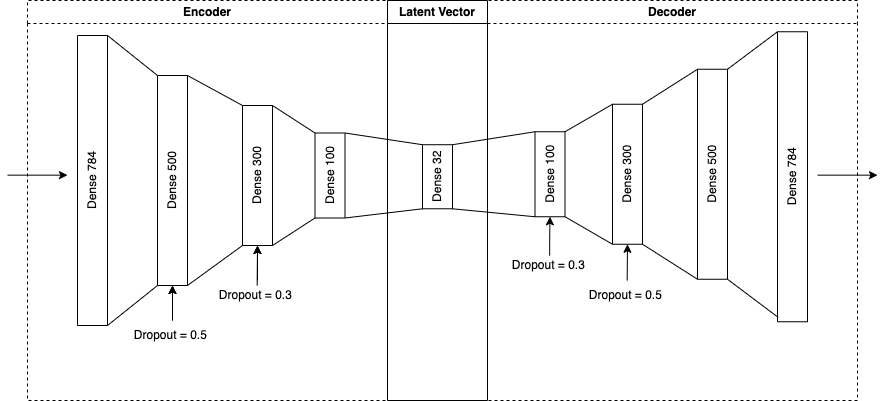
\includegraphics[width=14cm]{img/tesis/autoencoder_arquitectura.png}
    \caption{Autoencoder: Esta arquitectura se utiliza para obtener la representación de baja dimensionalidad de los datos.}
    \label{fig:autoencoder_arquitectura}
\end{figure}

La Figura \ref{fig:autoencoder_arquitectura} muestra la arquitectura que se utilizará para el entrenamiento del \textit{Autoencoder} utilizado para la reducción de dimensionalidad de las imágenes de \textit{Fashion MNIST}. Los parámetros en los distintos experimentos se detallan en \ref{table:autoencoder_parameters}.

\subsection{Oneshot}

\begin{figure}[ht]
    \centering
    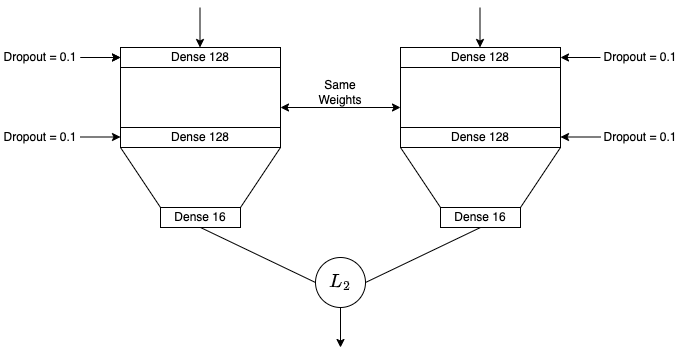
\includegraphics[width=14cm]{img/tesis/oneshot_arquitectura.png}
    \caption{Oneshot: Esta arquitectura se utiliza para el aprendizaje de la métrica de distancia necesaria para un DPP.}
    \label{fig:oneshot_arquitectura}
\end{figure}


La Figura \ref{fig:oneshot_arquitectura} muestra la arquitectura que se utilizará para el entrenamiento de la red siamesa \textit{Oneshot} que define una métrica de distancia entre pares de ejemplos de \textit{Fashion MNIST}. El entrenamiento se realiza utilizando \textit{contrastive loss} y los parámetros utilizados en los distintos experimentos se detallan en \ref{table:oneshot_parameters}.

\subsection{DPP NET}

\begin{figure}[ht]
    \centering
    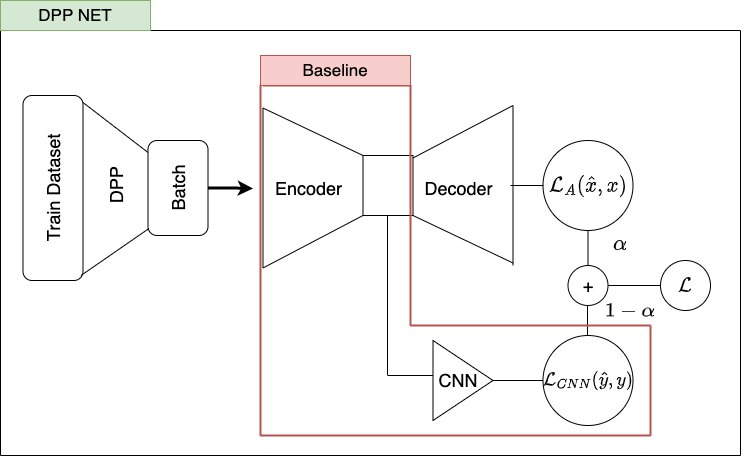
\includegraphics[width=12cm]{img/tesis/baseline_dppnet.png}
    \caption{Baseline y DPP NET: Esta figura muestra la arquitectura del baseline con el que se compararán los resultados de DPP NET.}
    \label{fig:baseline_dpp_net}
\end{figure}

La Figura \ref{fig:dpp_net} detalla el esqueleto utilizado para el entrenamiento de la red DPP NET. La arquitectura del \textit{Autoencoder} es la misma presentada en Figura \ref{fig:autoencoder_arquitectura} y la red encargada de clasificar los ejemplos es la presentada en Figura \ref{fig:conv}. Para ser comparables ambas metodologías, el \textit{baseline} se re-define como la Figura \ref{fig:baseline_dpp_net}. Los parámetros utilizados en los experimentos se detallan en Tabla \ref{table:dppnet_parameters}.

